% Part IV: learning (sections 9-10)
\addcontentsline{toc}{part}{Part IV \quad Learning}
\section{Maximum likelihood, EM, and generalised EM}\label{sec:em}

\subsection{Likelihood and its target}

A model is a family of densities $p_\theta$ indexed by parameters $\theta$. Given independent data $y_1,\dots,y_n$,
the \emph{log-likelihood} $\mathcal L(\theta)=\sum_k\log p_\theta(y_k)$ scores how well $\theta$ explains them, and
the \emph{maximum likelihood estimate} (MLE) maximises it. Two examples we use.
For a Gaussian, the MLE of the mean is the sample mean and of the variance the mean squared deviation. For
a clean AR(1) chain, $\mathcal L(\rho,q)=\sum_i\log\N(a_{i+1};\rho a_i,q)$, which is a least-squares problem:
$\hat\rho=\sum_ia_ia_{i+1}/\sum_ia_i^2$ and $\hat q$ the mean squared residual.

What does the MLE converge to? Divide $\mathcal L$ by $n$: by the law of large numbers it approaches
$\E_{\rm true}[\log p_\theta(y)]$. Compare with the \emph{Kullback--Leibler divergence}
\[
  \KL(p\,\|\,q)=\int p\log\frac pq\;\ge0,\qquad\text{with equality only if }p=q,
\]
(the inequality is Jensen's: $\E_p\log(q/p)\le\log\E_p(q/p)=\log1=0$). Since
$\E_{\rm true}\log p_\theta=-\KL(p_{\rm true}\|p_\theta)+\text{const}$, maximising likelihood is minimising the
divergence from the truth to the model.

\begin{keyidea}
If the truth is in the family, the MLE finds it (consistency). If it is not, the MLE converges to the member
\emph{closest} to the truth in KL divergence, and stays there: the remaining error is an asymptotic bias that
no amount of data removes. Separating ``needs more data'' from ``needs a better family'' is what several of our
predictions test (E33 P1, E35 P2).
\end{keyidea}

\subsection{Latent variables and the evidence lower bound}

Often the model describes a pair $(a,x)$ but we observe only $x$: the clean chain behind the noised one, the
component label behind a mixture draw. The likelihood is then the \emph{evidence}
$\log p_\theta(x)=\log\int p_\theta(x,a)\dd a$, the logarithm of an integral, awkward to maximise. The way in is a
lower bound. For \emph{any} density $q(a)$, by Jensen's inequality,
\begin{equation}\label{eq:elbo}
  \log p_\theta(x)=\log\int q(a)\frac{p_\theta(x,a)}{q(a)}\dd a\;\ge\;\int q(a)\log\frac{p_\theta(x,a)}{q(a)}\dd a=:F(q,\theta).
\end{equation}
$F$ is the \emph{evidence lower bound} (ELBO). The gap is exactly a divergence: writing
$p_\theta(x,a)=p_\theta(a\mid x)p_\theta(x)$ inside $F$ gives
\begin{equation}\label{eq:elbogap}
  \log p_\theta(x)=F(q,\theta)+\KL\big(q\,\|\,p_\theta(\cdot\mid x)\big),
\end{equation}
so the bound is tight exactly when $q$ is the posterior.

\subsection{The EM algorithm}

EM climbs $F$ by alternating over its two arguments.
\begin{itemize}
\item \textbf{E-step.} Set $q=p_{\theta_{\rm old}}(a\mid x)$, the posterior under the current parameters. By
  \eqref{eq:elbogap} this closes the gap: $F(q,\theta_{\rm old})=\log p_{\theta_{\rm old}}(x)$.
\item \textbf{M-step.} Maximise $F(q,\theta)$ over $\theta$ with $q$ fixed. The term $-\int q\log q$ does not involve
  $\theta$, so this maximises
  \begin{equation}\label{eq:Q}
    Q(\theta\mid\theta_{\rm old})=\E_{a\sim p_{\theta_{\rm old}}(\cdot\mid x)}\big[\log p_\theta(x,a)\big],
  \end{equation}
  the expected \emph{complete-data} log-likelihood.
\end{itemize}

\begin{proposition}[EM never decreases the evidence]
$\log p_{\theta_{\rm new}}(x)\ge\log p_{\theta_{\rm old}}(x)$.
\end{proposition}
\begin{proof}
$\log p_{\theta_{\rm new}}(x)\ge F(q,\theta_{\rm new})\ge F(q,\theta_{\rm old})=\log p_{\theta_{\rm old}}(x)$: the bound, then the M-step,
then the tight E-step.
\end{proof}

The proof also shows what is \emph{needed}: any $\theta_{\rm new}$ with $Q(\theta_{\rm new}\mid\theta_{\rm old})\ge Q(\theta_{\rm old}\mid\theta_{\rm old})$
works. A decrease of the evidence is therefore always a bug or a too-generous approximate step, never a feature
of EM. Our code records every decrease rather than stopping on it.

\begin{example}[a mixture of two Gaussians]
Data $y_k$ come from component $c\in\{1,2\}$ with probability $w_c$, then $y_k\sim\N(\mu_c,\sigma_c^2)$. The label is
latent. The E-step computes the \emph{responsibilities}, the posterior probabilities of the labels,
\[
  r_{kc}=\frac{w_c\,\N(y_k;\mu_c,\sigma_c^2)}{\sum_{c'}w_{c'}\,\N(y_k;\mu_{c'},\sigma_{c'}^2)};
\]
the M-step sets $w_c$ to the average responsibility and $\mu_c,\sigma_c^2$ to responsibility-weighted means and
variances. Figure~\ref{fig:em} shows the evidence rising at every iteration, with a long plateau: when the
components overlap, EM can crawl.
\end{example}

\begin{figure}[h]\centering
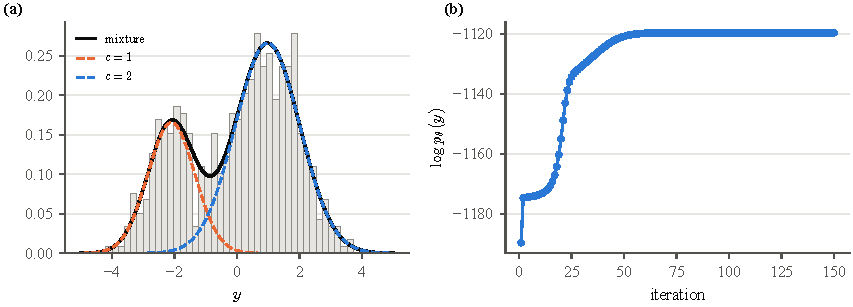
\includegraphics{primer-em.pdf}
\caption{EM on a two-component mixture ($600$ draws). (a) The fitted mixture and its components. (b) The
log-evidence per iteration: never decreasing, but slow while the components are still entangled.}
\label{fig:em}
\end{figure}

\subsection{Generalised EM: the family}

Exact E- and M-steps are luxuries. The variants keep the monotone climb by relaxing one of them.
\begin{itemize}
\item \textbf{Generalised EM (GEM).} Any parameter with higher $Q$ instead of the maximiser. Our kernels accept an
  M-step only if $Q$ did not decrease, and otherwise return the old parameters.
\item \textbf{ECM} (expectation conditional maximisation). Maximise $Q$ over blocks of parameters in turn. The
  innovation-mixture kernel updates its correlation, then its components.
\item \textbf{Gradient EM.} One or a few gradient steps on $Q$, with a line search; the neural (MDN) kernel does
  this with Adam steps and backtracking.
\item \textbf{Variational EM.} When the exact posterior is intractable (two-dimensional fields), restrict $q$ to a
  simple family and maximise $F$ over it; the bound \eqref{eq:elbo} is no longer tight, so one maximises a bound
  rather than the evidence.
\item \textbf{Monte Carlo and stochastic EM.} Replace the expectation in \eqref{eq:Q} by an average over posterior
  samples; online EM updates the expected statistics as data stream in.
\end{itemize}
All are instances of \emph{minorise--maximise}: $F(q,\cdot)$ is a function below $\log p_\theta(x)$ that touches it at
$\theta_{\rm old}$, and any increase of the minoriser is an increase of the target.

\subsection{EM on chains (Baum--Welch)}\label{sec:emchain}

For a hidden Markov chain, $\log p_\theta(x,a)=\log\mu_\theta(a_1)+\sum_i\log K_\theta(a_{i+1}\mid a_i)+\sum_i\log\ell_i(a_i)$. Taking
the posterior expectation, the only part that involves the kernel is
\begin{equation}\label{eq:Qchain}
  Q(\theta)=\iint\Xi(a,a')\,\log K_\theta(a'\mid a)\dd a\dd a'+\text{(site-one term)},\qquad
  \Xi=\sum_{\text{sequences}}\sum_i\xi_i ,
\end{equation}
with $\xi_i$ the pair marginals \eqref{eq:pair}. $\Xi(a,a')$ is the \emph{expected number of transitions} from $a$ to
$a'$, and the E-step is one forward--backward pass per sequence. The M-step is a weighted fit of the kernel to
these soft counts. With clean data the posterior is a point mass and $\Xi$ is just the histogram of observed
transitions: no E-step at all.

If the kernel is an exponential family in its parameters for each source $a$,
$\log K_\theta(a'\mid a)=\theta\cdot B(a')+c(a,a')-\log Z_\theta(a)$, then $Q$ is a linear function of $\theta$ minus a sum
of log-normalisers, hence concave, and its gradient is
\begin{equation}\label{eq:expfamgrad}
  \nabla_\theta Q=\sum_{a}\Big[\sum_{a'}\Xi(a,a')B(a')-N(a)\,\E_{K_\theta(\cdot\mid a)}[B]\Big],\qquad N(a)=\sum_{a'}\Xi(a,a'):
\end{equation}
expected statistics under the data minus expected statistics under the model, source by source. The
tilted-walk kernel of \S\ref{sec:synthesis} is of this kind.

\subsection{Fisher's identity and Boltzmann learning}\label{sec:fisherid}

\begin{proposition}[Fisher's identity]
$\nabla_\theta\log p_\theta(x)=\E_{a\sim p_\theta(\cdot\mid x)}\big[\nabla_\theta\log p_\theta(x,a)\big]$.
\end{proposition}
\begin{proof}
$\nabla p_\theta(x)=\int\nabla p_\theta(x,a)\dd a=\int p_\theta(x,a)\nabla\log p_\theta(x,a)\dd a$; divide by $p_\theta(x)$.
\end{proof}
Three uses. The gradient of the evidence costs one E-step. At a fixed point of EM the gradient of $Q$ vanishes,
so EM converges to stationary points of the evidence. And it gives Boltzmann learning: for an energy model
$p_\theta(a)=e^{-\En_\theta(a)}/\Zp_\theta$ seen through a likelihood, $\nabla\log\Zp_\theta=-\E_{p_\theta}[\nabla\En_\theta]$, so
\begin{equation}\label{eq:boltzmann}
  \nabla_\theta\log p_\theta(x)=-\underbrace{\E_{a\mid x}[\nabla\En_\theta(a)]}_{\text{positive phase}}+\underbrace{\E_{a\sim p_\theta}[\nabla\En_\theta(a)]}_{\text{negative phase}} .
\end{equation}
The positive phase pulls the energy down where the data's posterior sits; the negative phase pushes it up where
the model already puts mass. For an undirected chain both phases are pair expectations computable by transfer
matrices. For a directed kernel the negative phase becomes the per-source expectation in \eqref{eq:expfamgrad}, and
no chain-wide partition function appears.

\subsection{How fast EM goes}

Near its limit EM converges geometrically, with a rate equal to the \emph{fraction of missing information}: the
share of the complete-data information about $\theta$ that the observations do not carry (\S\ref{sec:fisher}).
When noise hides most of the clean chain, that fraction is close to one and EM needs many iterations. This is
why our EM runs a ladder of checkpoints up to $1200$ iterations, selects the checkpoint on held-out data, and
flags runs whose selected checkpoint is the last one.

\paragraph{Check yourself.}
\begin{enumerate}[label=\thesection.\arabic*,leftmargin=2.2em]
\item Why does the M-step of the mixture produce responsibility-weighted averages?
\item An approximate M-step returns parameters with a \emph{lower} $Q$ than before. What can happen to the evidence?
\end{enumerate}

\section{Fisher information, Cram\'er--Rao, and quasi-likelihood}\label{sec:fisher}

\subsection{Fisher information}

The parameter score $U_\theta(x)=\partial_\theta\log p_\theta(x)$ has mean zero at the true parameter:
$\E U=\int\partial_\theta p_\theta=\partial_\theta\int p_\theta=0$. Its variance is the \emph{Fisher information},
\begin{equation}\label{eq:fisher}
  I(\theta)=\E\big[U_\theta(x)^2\big]=-\E\big[\partial_\theta^2\log p_\theta(x)\big],
\end{equation}
the second form following by differentiating $\E U=0$ once more. It is the curvature of the expected
log-likelihood at its peak: a sharp peak means the data pin the parameter down. For $n$ independent
observations it adds up to $nI(\theta)$.

\begin{proposition}[Cram\'er--Rao]
Any unbiased estimator $\hat\theta$ of $\theta$ from $n$ observations has $\Var(\hat\theta)\ge1/\big(nI(\theta)\big)$.
\end{proposition}
\begin{proof}
Differentiate $\E_\theta\hat\theta=\theta$: $\int\hat\theta\,\partial_\theta p_\theta=1$, i.e.\ $\Cov(\hat\theta,U)=1$ for the total score $U$, whose
variance is $nI$. By Cauchy--Schwarz, $1=\Cov(\hat\theta,U)^2\le\Var(\hat\theta)\,nI(\theta)$.
\end{proof}
The MLE attains the bound for large $n$: $\sqrt n(\hat\theta-\theta)$ becomes Gaussian with variance $1/I(\theta)$. With
several parameters $I$ is a matrix and the bound is its inverse.

\begin{example}[AR(1)]
With the innovation variance $q$ known, $\partial_\rho\log\N(a';\rho a,q)=(a'-\rho a)a/q$, whose mean square under the
stationary chain is $\E[\varepsilon^2]\E[a^2]/q^2=1/q$. So each clean transition carries information $1/(1-\rho^2)$ about
$\rho$, and $\Var\hat\rho\approx(1-\rho^2)/n$ from $n$ transitions.
\end{example}

\subsection{Information lost to noise}

When only noised data are seen, Fisher's identity says the observed score is the posterior average of the
complete-data score, $U_{\rm obs}=\E[U_{\rm complete}\mid x]$. The law of total variance then splits the information:
\begin{equation}\label{eq:missinginfo}
  I_{\rm complete}=I_{\rm obs}+\underbrace{\E\big[\Var(U_{\rm complete}\mid x)\big]}_{I_{\rm missing}},
\end{equation}
the \emph{missing information principle}. Noise moves information from the first term to the second.

The channel does this selectively, and Hermite polynomials say how. A parameter that changes only the
degree-$n$ Hermite content of the law enters the noised density \eqref{eq:noisedgc} through $c_ne^{-nt}$. Its score
is then about $e^{-nt}(\partial_\theta c_n)H_n(x)/n!$, and its information about $e^{-2nt}(\partial_\theta c_n)^2/n!$. A
covariance coordinate (degree $2$) loses information like $e^{-4t}$; a shape coordinate such as the kurtosis
(degree $4$) like $e^{-8t}$. Since the number of sequences needed for a fixed accuracy is inversely
proportional to the information, it grows like $e^{4t}$ and $e^{8t}$ respectively.

\begin{inproject}
E12b measured exactly this (frozen 1 October): the sample size needed for a fixed accuracy grows with the
noise level with log-slope $4.95$ (interval $3.09$ to $6.83$) for the covariance coordinate, and for the shape
coordinate the requirement is unresolved beyond $t=0.8$ even at $8192$ sequences (slope above $6.7$). Both agree
with the exact information curve, whose local slopes on these levels are $3.8$--$3.9$ and $6.1$--$6.9$; the
asymptotic $4$ and $8$ are reached only at larger $t$.
\end{inproject}

\subsection{Quasi-likelihood: using a wrong model on purpose}

Sometimes we maximise a likelihood we know to be wrong because it is convenient. This is sound if the
\emph{estimating equation} is right. Let $g(\theta)$ be the gradient of the convenient objective. If its mean
under the \emph{true} law vanishes at the target value $\theta^\star$, the solution of $g(\hat\theta)=0$ converges to
$\theta^\star$, with variance given by the \emph{sandwich} $A^{-1}BA^{-1}$, where $A=-\E[\partial g]$ and $B=\Var g$. When the
objective is the true log-likelihood, $A=B=I$ (the information equality) and the sandwich reduces to the
Cram\'er--Rao bound. When the model is simply misspecified, the MLE converges to the KL projection of the
truth (White's theorem) and the sandwich gives honest error bars around it.

The quasi-likelihood that matters here is the Gaussian one. For a zero-mean sequence with model covariance
$\Sigma_\theta$,
\[
  \ell(\theta)=-\tfrac12\log\det\Sigma_\theta-\tfrac12x\T\Sigma_\theta^{-1}x,\qquad
  \E_{\rm true}\,\ell(\theta)=-\tfrac12\log\det\Sigma_\theta-\tfrac12\operatorname{tr}\big(\Sigma_\theta^{-1}\Sigma^\star\big).
\]
It depends on the data only through their covariance, and its expectation is maximised at $\Sigma_\theta=\Sigma^\star$
whatever the true law is. A Gaussian model is therefore consistent for everything the covariance determines
(the correlation, the variance) and blind to everything else.

\begin{keyidea}
Fitting a Gaussian-innovation kernel by EM on noised chains is a Gaussian quasi-likelihood: it converges to
the covariance twin and its denoiser lands on the linear floor, never below it. To beat the floor, the kernel
family must be able to represent non-Gaussian structure. That is why the project's estimator uses mixture,
tilted and pair-energy kernels.
\end{keyidea}

\subsection{Pseudo-likelihood: avoiding the partition function}

For a Markov random field the likelihood needs $\Zp_\theta$, an integral over all configurations. Besag's
\emph{pseudo-likelihood} replaces the joint density by the product of each site's conditional law given its
neighbours, $\prod_ip_\theta(a_i\mid a_{i-1},a_{i+1})$; each factor is normalised over one site only, so no $\Zp_\theta$
appears. It is consistent but less efficient; composite likelihoods generalise it. On a chain the
exact likelihood is no harder: written with a directed kernel \eqref{eq:chain}, it needs only one normaliser per
source value, because the ground-state transform (\S\ref{sec:transfer}) has absorbed the partition function. This
is the special luck of one dimension that the learned pair energy exploits.

\paragraph{Check yourself.}
\begin{enumerate}[label=\thesection.\arabic*,leftmargin=2.2em]
\item For $n$ draws from $\N(\mu,1)$, what is the Fisher information about $\mu$, and which estimator attains the
  Cram\'er--Rao bound?
\item Why can a Gaussian quasi-likelihood never learn the kurtosis of the innovations?
\end{enumerate}
